
\section{Introduction}

The intention of the following SoC interconnect standard is to be
simple and efficient with respect to implementation resources and
transaction latency.

SimpCon is a fully synchronous standard for on-chip
interconnections. It is a point-to-point connection between a master
and a slave. The master starts either a read or write transaction.
Master commands are single cycle to free the master to continue on
internal operations during an outstanding transaction. The slave has
to register the address when needed for more than one cycle. The
slave also registers the data on a read and provides it to the
master for more than a single cycle. This property allows the master
to delay the actual read if it is busy with internal operations.

The slave signals the end of the transaction through a novel
\emph{ready counter} to provide an early notification. This early
notification simplifies the integration of peripherals into
pipelined masters.

Slaves can also provide several levels of pipelining. This feature
is announced by two static output ports (one for read and one write
pipeline levels).

Off-chip connections (e.g.\ main memory) are device specific and
need a slave to perform the translation. Peripheral interrupts are
not covered by this specification.

\subsection{Features}

\begin{itemize}
    \item Master/slave point-to-point connection
    \item Synchronous operation
    \item Read and write transactions
    \item Early pipeline release for the master
    \item Pipelined transactions
    \item Open-source specification
    \item Low implementation overheads
\end{itemize}

\subsection{Basic Read Transaction}

Figure~\ref{fig:sc:basic:rd} shows a basic read transaction for a
slave with one cycle latency. The acknowledge signals are omitted
from the figure. In the first cycle, the address phase, the
\sign{rd} signals the slave to start the read transaction. The
address is registered by the slave. During the following cycle, the
read phase, the slave performs the read and registers the data. Due
to the register in the slave the data is available in the third
cycle, the result phase. To simplify the master, \sign{rd\_data}
stays valid till the next read request response. It is therefore
possible for a master to issue a pre-fetch command early. When the
pre-fetched data arrives to early it is still valid when the master
actually wants to read it.

\begin{figure}
    \centering
    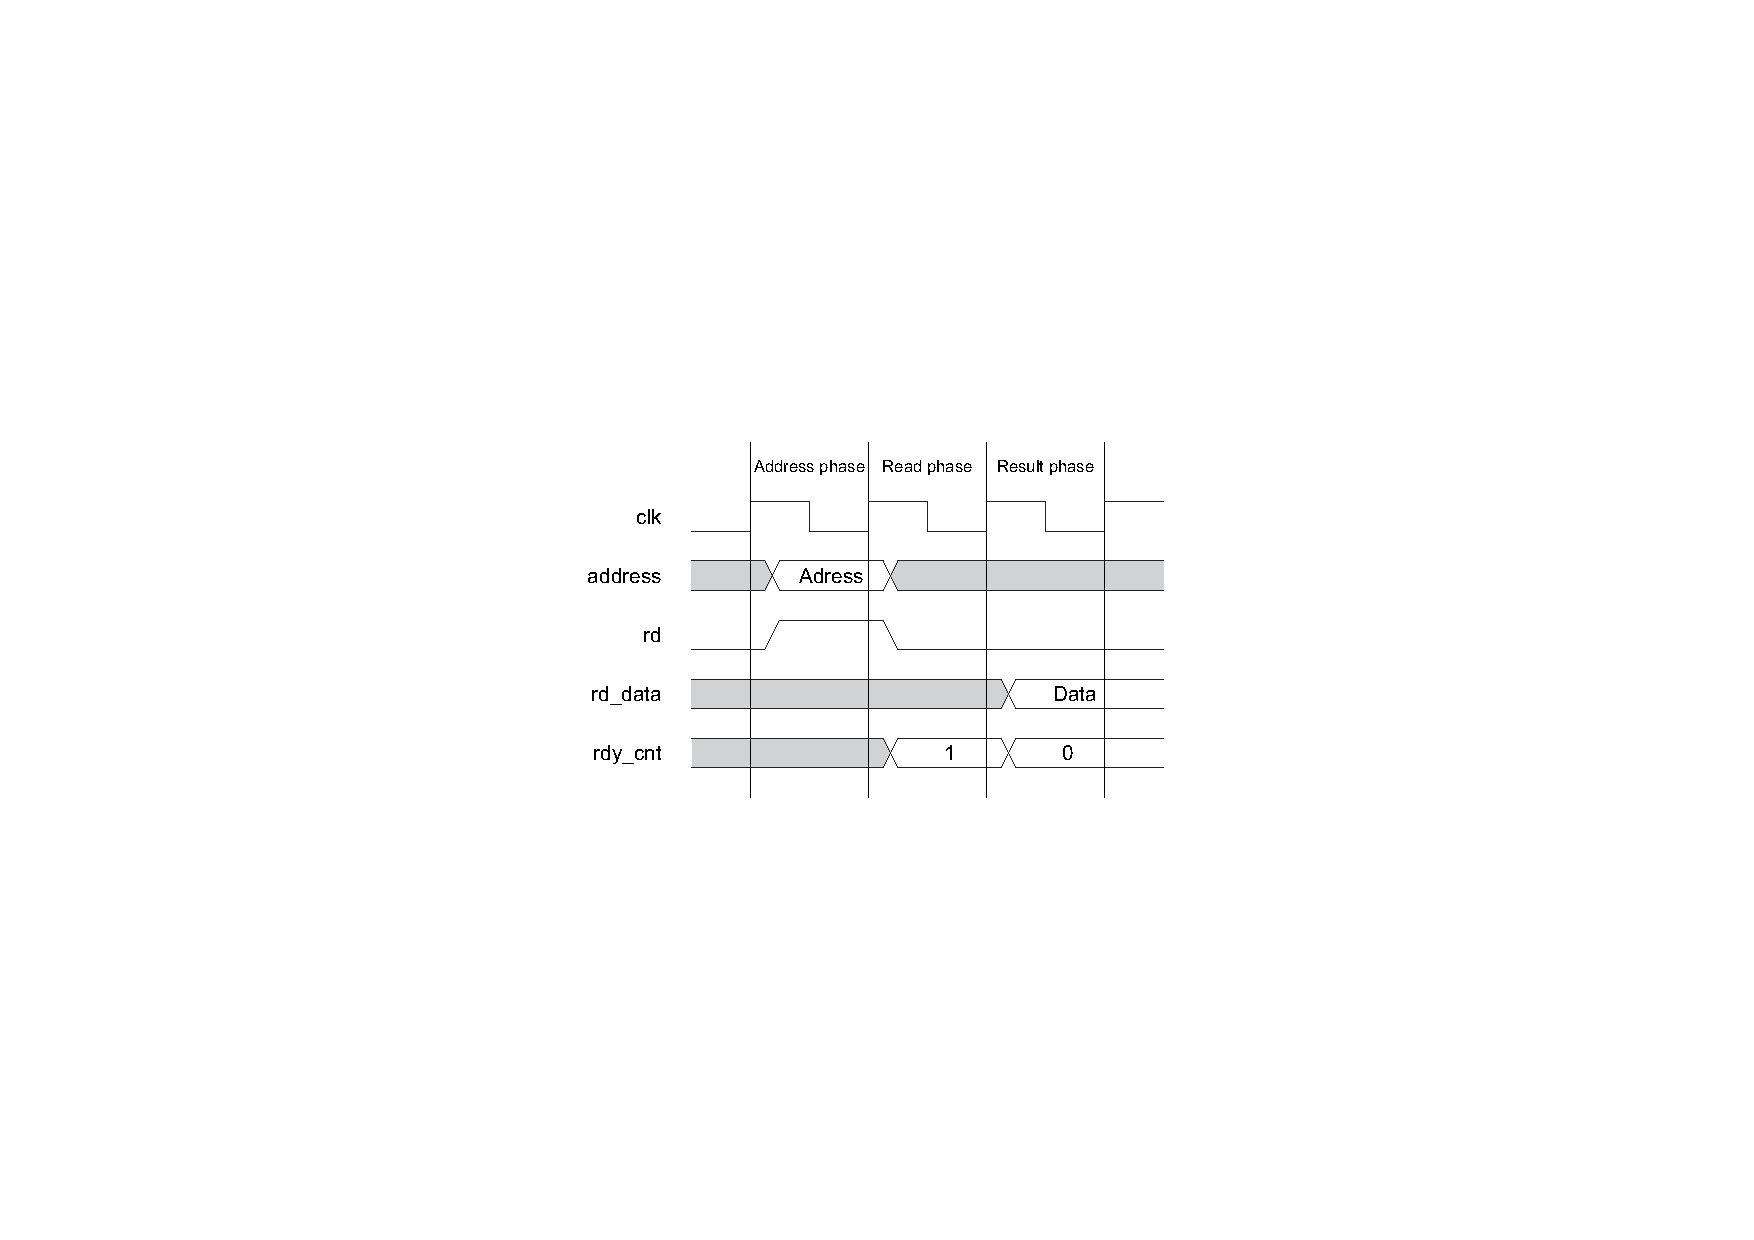
\includegraphics[scale=\scgrsc]{\scgrp/sc_basic_rd}
    \caption{Basic read transaction}
    \label{fig:sc:basic:rd}
\end{figure}

\subsection{Basic Write Transaction}

A write transaction consists of a single cycle address/command phase
started by assertion of \sign{wr} where the address and the write
data are valid. \sign{address} and \sign{wr\_data} are usually
registered by the slave. The end of the write cycle is signalled to
the master by the slave with \sign{rdy\_cnt}. See
Section~\ref{sec:ack} and an example in Figure~\ref{fig:sc:wr:ws}.

\section{SimpCon Signals}

This sections defines the signals used by the SimpCon connection.
Some of the signals are optional and may not be present on a
peripheral device.

All signals are a single direction point-to-point connection between
a master and a slave. The signal details are described by the device
that drives the signal. Table~\ref{tab:sc:signals} lists the signals
that define the SimpCon interface. The column Direction indicates
wether the signal is driven by the master or the slave.

\begin{table}
    \centering

    \begin{tabular}{lrlll}
        \toprule
        Signal & Width & Direction & Required & Description \\
        \midrule
        \sign{address} & 1--32 & Master & No & Address lines from the
        master\\
        & & & & to the slave port\\
        \sign{wr\_data} & 32 & Master & No & Data lines from the
        master\\
        & & & & to the slave port\\
        \sign{rd} & 1 & Master & No & Start of a read transaction \\
        \sign{wr} & 1 & Master & No & Start of a write transaction \\
        \sign{rd\_data} & 32 & Slave & No & Data lines from the
        slave\\
        & & & & to the master port\\
        \sign{rdy\_cnt} & 2 & Slave & Yes & Transaction end signalling \\
        \sign{rd\_pipeline\_level} & 2 & Slave & No & Maximum pipeline
        level\\
        & & & & for read transactions \\
        \sign{wr\_pipeline\_level} & 2 & Slave & No & Maximum pipeline
        level\\
        & & & & for write transactions \\
        \bottomrule

    \end{tabular}
    \caption{SimpCon port signals}
    \label{tab:sc:signals}

\end{table}



\subsection{Master Signal Details}

This section describes the signals that are driven by the master to
initiate a transaction.

\subsubsection{address}

Master addresses represent word addresses as offsets in the slaves
address range. \sign{address} is valid a single cycle either with
\sign{rd} for a read transaction or with \sign{wr} and
\sign{wr\_data} for a write transaction.

The number of bits for \sign{address} depend on the slaves address
range. For a single port slave \sign{address} can be omitted.

\subsubsection{wr\_data}

The \sign{wr\_data} signals carry the data for a write transaction.
It is valid for a single cycle together with \sign{address} and
\sign{wr}. The signal is typically 32 bits wide. Slaves can ignore
upper bits when the slave port is less than 32 bits.

\subsubsection{rd}

The \sign{rd} signal is asserted a single clock cycle to start a
read transaction. \sign{address} has to be valid in the same cycle.

\subsubsection{wr}

The \sign{wr} signal is asserted a single clock cycle to start a
write transaction. \sign{address} and \sign{wr\_data} have to be
valid in the same cycle.

\subsubsection{sel\_byte}

The \sign{sel\_byte} signal is reserved for future versions of the
SimpCon specification to add individual byte enables.

\subsection{Slave Signal Details}

This section describes the signals that are driven by the slave as a
response to transaction initiated by the master.

\subsubsection{rd\_data}

The \sign{wr\_data} signals carry the result for a read transaction.
The data is valid when \sign{rdy\_cnt} reaches 0 and stays valid
till a new read result is available. The signal is typically 32 bits
wide. Slaves that provide less than 32 bits should pad the upper
bits with 0.

\subsubsection{rdy\_cnt}

The \sign{rdy\_cnt} signal provides the number of cycles till the
pending transaction will finish. A 0 means that either read data is
available or a write transaction has been finished. Values of 1 and
2 mean the the transaction will finish in at least 1 or 2 cycles.
The maximum value is 3 and means the the transaction will finish in
3 or \emph{more} cycles. Note that not all values have to be used in
a transaction. Each monotonic sequence of \sign{rdy\_cnt} values is
legal.

\subsubsection{rd\_pipeline\_level}

The static \sign{rd\_pipeline\_level} provides the master with the
read pipeline level of the slave. The signal has to be constant to
enable the synthesizer to optimize the pipeline level dependent
state machine in the master.


\subsubsection{wr\_pipeline\_level}

The static \sign{wr\_pipeline\_level} provides the master with the
write pipeline level of the slave. The signal has to be constant to
enable the synthesizer to optimize the pipeline level dependent
state machine in the master.

\section{Slave Acknowledge}
\label{sec:ack}

Flow control between the slave and the master is usually done by a
single signal in the form of \emph{wait} or \emph{acknowledge}. The
\sign{ack} signal, e.g.\ in the Wishbone specification, is set when
the data is available or the write operation has finished. However,
for a pipelined master it can be of interest to know it
\emph{earlier} when a transaction will finish.


For many slaves, e.g.\ an SRAM interface with fixed wait states,
this information is available inside the slave. In the SimpCon
interface this information is communicated to the master through the
two bit ready counter (\sign{rdy\_cnt}). \sign{rdy\_cnt} signals the
number of cycles till the read data will be available or the write
transaction will be finished. Value 0 is equivalent to an \emph{ack}
signal and 1, 2, and 3 are equivalent to a wait request with the
distinction that the master knows how long the wait request will
last.

To avoid too many signals at the interconnect \sign{rdy\_cnt} has a
width of two bits. Therefore, the maximum value of 3 has the special
meaning that the transaction will finish in 3 or \emph{more} cycles.
As a result the master can only use the values 0, 1, and 2 to
release actions in its pipeline. If necessary an extension for a
longer pipeline is straightforward with a larger
\sign{rdy\_cnt}\footnote{The maximum value of the ready counter is
relevant for the early restart of a waiting master. A longer latency
from the slave e.g., for DDR SDRAM, will map to the maximum value of
the counter for the first cycles.}.

Idle slaves will keep the former value of 0 for \sign{rdy\_cnt}.
Slaves, that don't know in advance how many wait states are needed
for the transaction can produce sequences that omit any of the
numbers 3, 2, and 1. A simple slave can hold \sign{rdy\_cnt} on 3
until the data is available and set it than directly to 0. The
master has to handle those situations. Practically this reduces the
possibilities of pipelining and therefore the performance of the
interconnect. The master will read the data later, which is not an
issue as the data stays valid.

Figure~\ref{fig:sc:rd:ws} shows an example of a slave that needs
three cycles for the read to be processed. In cycle 1 the read
command and the address are set by the master. The slave registers
the address and sets \sign{rdy\_cnt} to 3 in cycle 2. The read takes
three cycles (2--4) during which \sign{rdy\_cnt} gets decremented.
In cycle 4 the data is available inside the slave and gets
registered. It is available in cycle 5 for the master and
\sign{rdy\_cnt} is finally 0. Both, the \sign{rd\_data} and
\sign{rdy\_cnt} will keep their value till a new transaction is
requested.

\begin{figure}
    \centering
    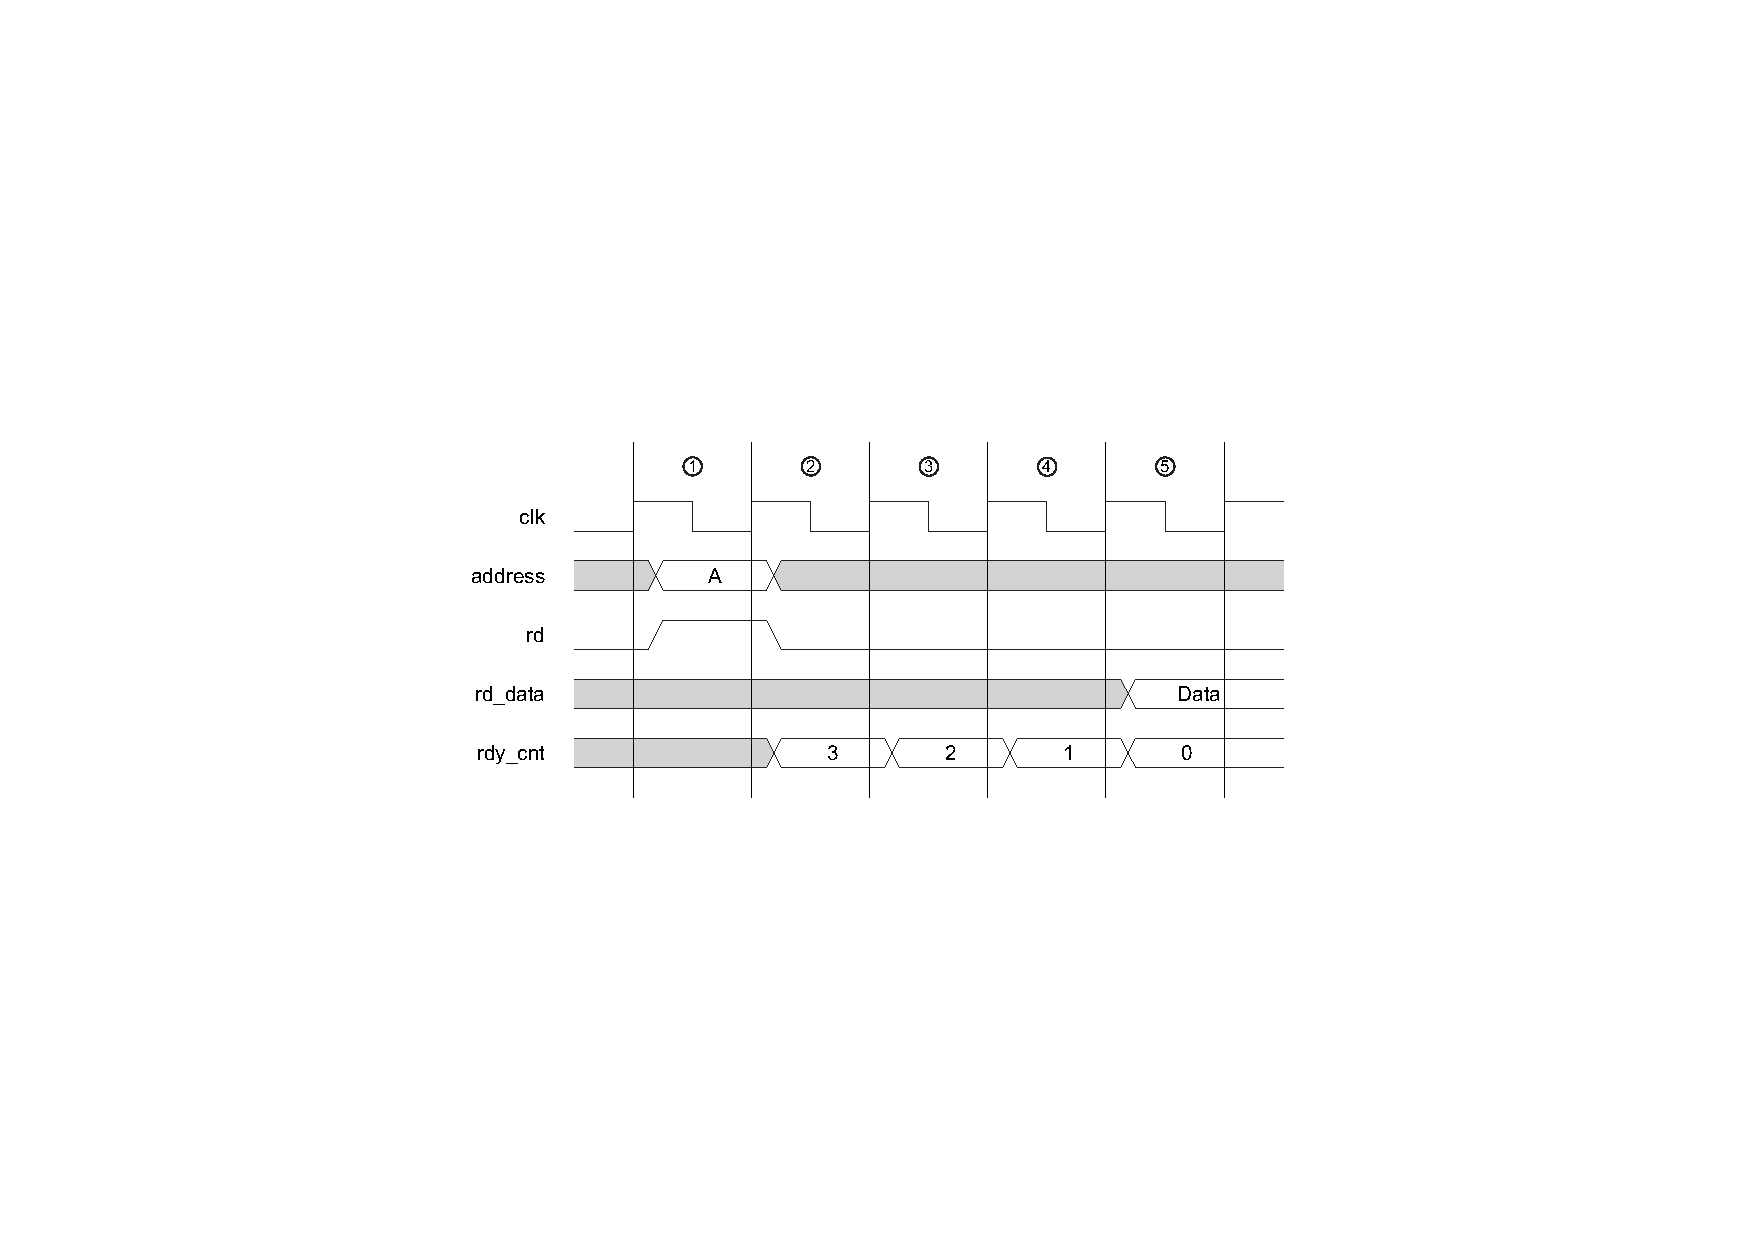
\includegraphics[scale=\scgrsc]{\scgrp/sc_rd_ws}
    \caption{Read transaction with wait states}
    \label{fig:sc:rd:ws}
\end{figure}


Figure~\ref{fig:sc:wr:ws} shows an example of a slave that needs
three cycles for the write to be processed. The address, the data to
be written and the write command are valid during cycle 1. The slave
registers the address and write data during cycle 1 and performs the
write operation during cycles 2--4. The \sign{rdy\_cnt} is
decremented and a non-pipelined slave can accept a new command after
cycle 4.

\begin{figure}
    \centering
    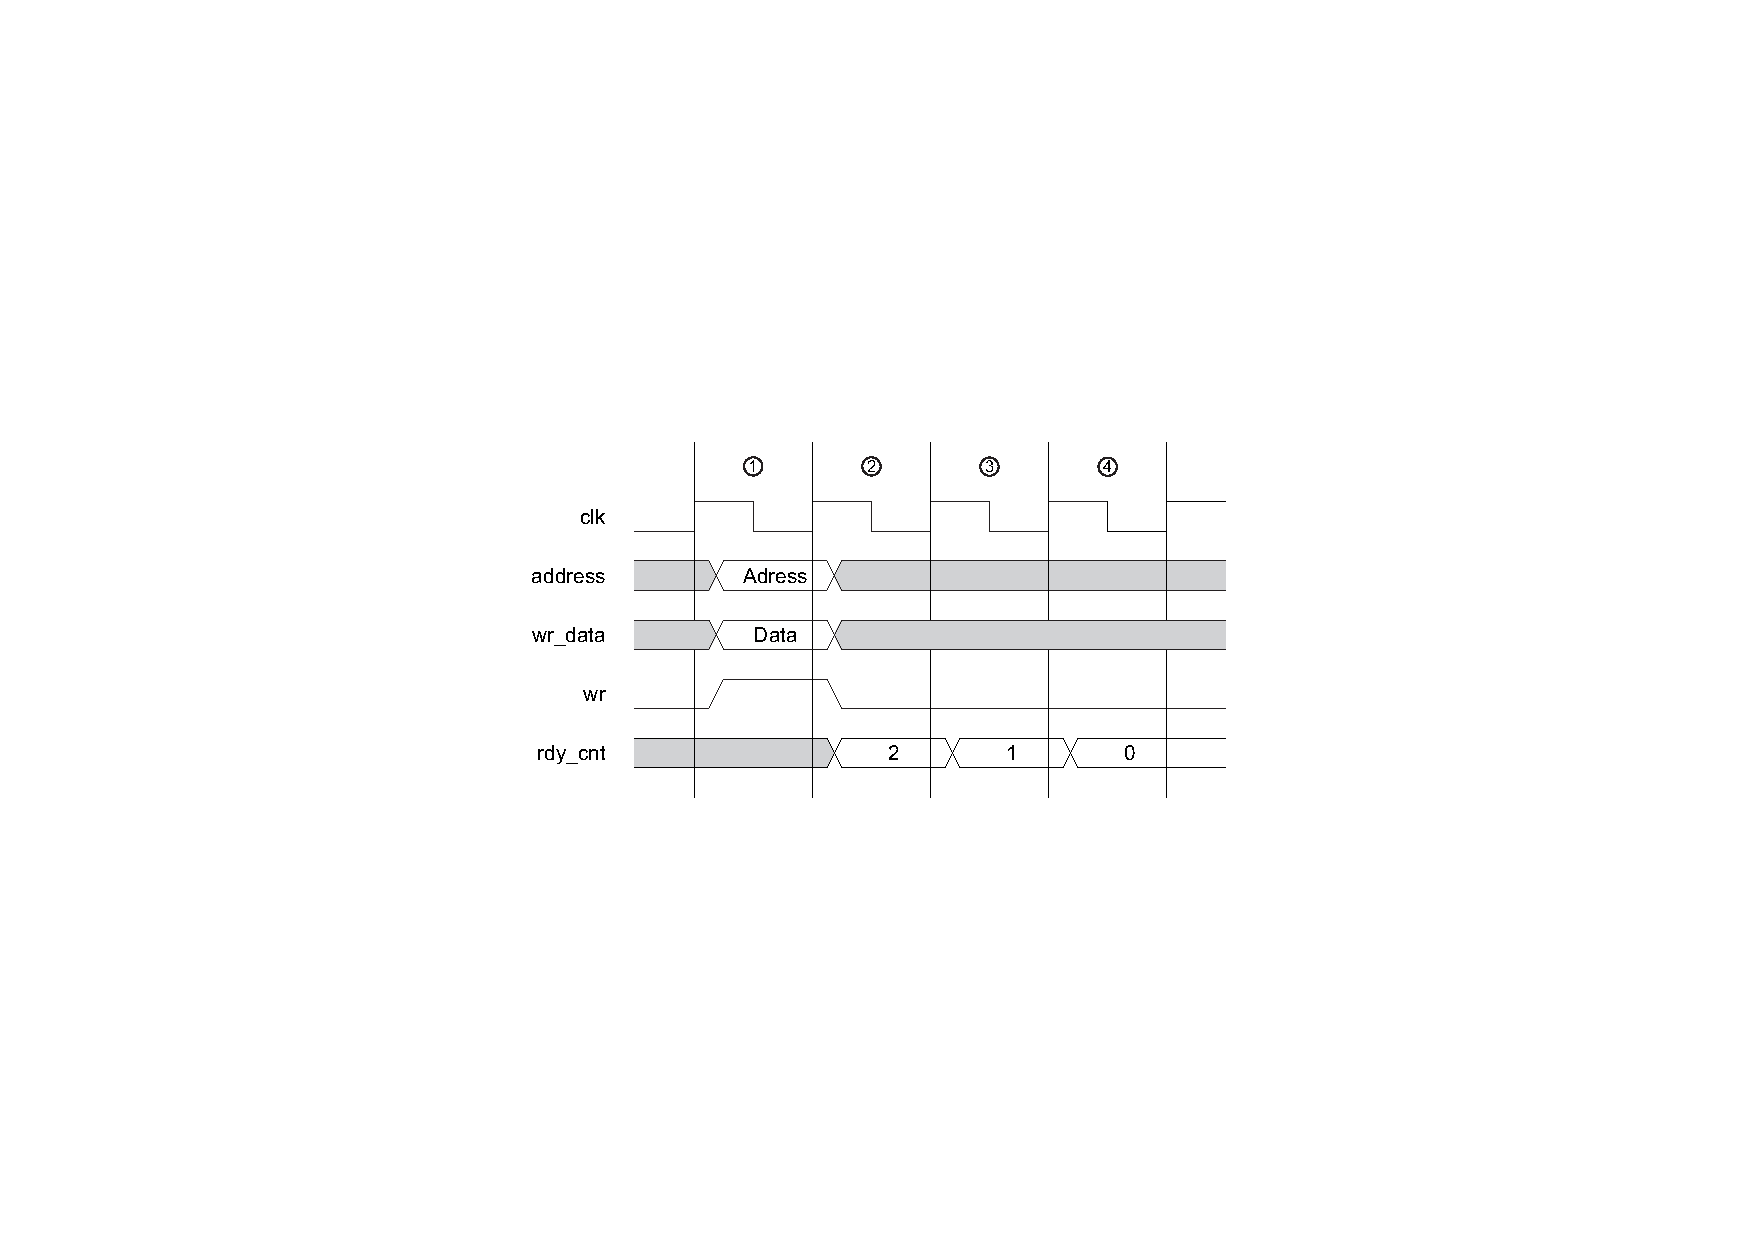
\includegraphics[scale=\scgrsc]{\scgrp/sc_wr_ws}
    \caption{Write transaction with wait states}
    \label{fig:sc:wr:ws}
\end{figure}



\section{Pipelining}

Figure~\ref{fig:sc:pipe:level} shows a read transaction for a slave
with four clock cycles latency. Without any pipelining the next read
transaction will start in cycle 7 after the data from the former
read transaction is read by the master. The three bottom lines show
when new read transactions (only the \sign{rd} signal is shown,
address lines are omitted from the figure) can be started for
different pipeline levels. With pipeline level 1 a new transaction
can start in the same cycle when the former read data is available
(in this example in cycle 6). At pipeline level 2 a new transaction
(either read or write) can start when \sign{rdy\_cnt} is 1, for
pipeline level 2 the next transaction can start at a \sign{rdy\_cnt}
of 2.

\begin{figure}
    \centering
    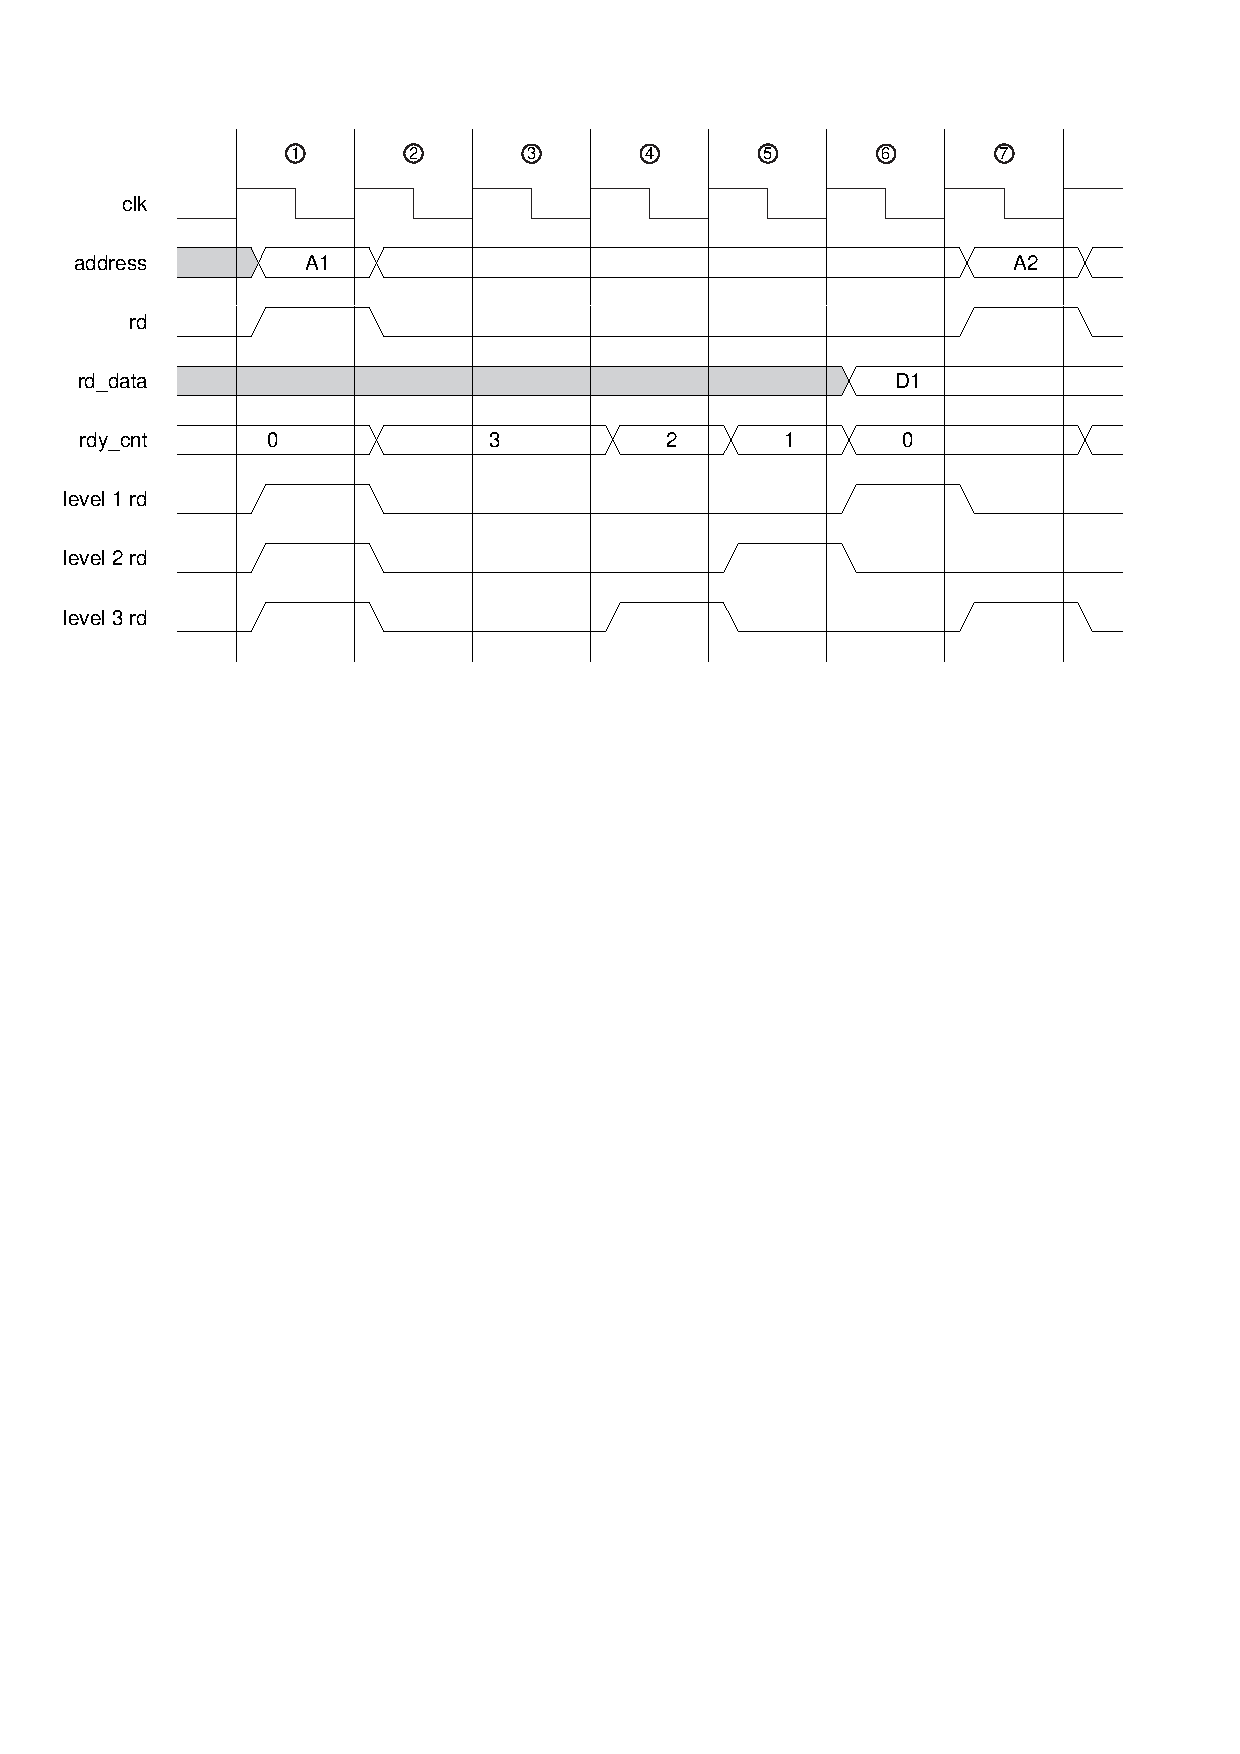
\includegraphics[scale=\scgrsc]{\scgrp/sc_pipe_level}
    \caption{Different pipeline levels for a read transaction}
    \label{fig:sc:pipe:level}
\end{figure}

The implementation of level 1 in the slave is trivial (just two more
transitions in the state machine). It is recommended to provide  at
least level 1 for read transactions. Level 2 is a little bit more
complex but usually no additional address or data registers are
necessary.

To implement level 3 pipelining in the slave at least an additional
address register is needed. However, to use level 3 the master has
to issue the request in the same cycle as \sign{rdy\_cnt} goes to 2.
That means this transition is combinatorial. We see in
Figure~\ref{fig:sc:pipe:level} that \sign{rdy\_cnt} value of 3 means
three or more cycles till the data is available and can therefore
not be used to trigger a new transaction. Extension to an even
deeper pipeline needs a wider \sign{rdy\_cnt}.


\subsection{Interconnect}

Although the definition of SimpCon is from a single master/slave
point-to-point viewpoint, all variations of multiple slave and
multiple master devices are possible.

\subsubsection{Slave Multiplexing}

To add several slaves to a single master \sign{rd\_data} and
\sign{rdy\_cnt} have to be multiplexed. Due to the fact that all
\sign{rd\_data} signals are already registered by the slaves a
single pipeline stage will be enough for a large multiplexer. The
selection of the multiplexer is also known at the transaction start
but needed at most in the next cycle. Therefore it can be registered
to further speed up the multiplexer.

%TODO: add a schematic for the master \sign{rd\_data} multiplexer.

\subsubsection{Master Multiplexing}

SimpCon defines no signals for the communication between a master
and an arbiter. However, it is possible to build a multi master
system with SimpCon. The SimpCon interface can be used as
interconnect between the masters and the arbiter and the arbiter and
the slaves. In this case the arbiter acts as slave for the master
and as master for the peripheral devices. An example of an arbiter
for SimpCon, where JOP and a VGA controller are two masters for a
shared main memory, can be found in \cite{jop:dma}. The same arbiter
is also used to build a chip-multiprocessor version of JOP.

The missing arbitration protocol in SimpCon results in the need to
queue $n-1$ requests in an arbiter for $n$ masters. However, this
additional hardware results in a zero cycle bus grant. The master,
which gets the bus granted, starts the slave transaction in the same
cycle as the original read/write request.

%TODO: add a timing diagram to explain this concept.


\section{Examples}

This section provides some examples for the application of the
SimpCon definition.

\subsection{IO Port}

TODO: Show how simple an IO port can be with SimpCon. We need no
addresses and can tie \sign{bsy\_cnt} to 0. We only need the
\sign{rd} or \sign{wr} signal to enable the port.

\subsection{SRAM interface}

The following example is taken from an implementation of SimpCon for
a Java processor. The processor is clocked with 100MHz and the main
memory consists of 15ns static RAMs. Therefore the minimum access
time for the RAM is two cycles. The slack time of 5ns forces us to
use output registers for the RAM address and write data and input
registers for the read data in the IO cells of the FPGA. These
registers fit nice with the intention of SimpCon to use registers
inside the slave.

Figure~\ref{fig:sc:sram} shows the memory interface for a
non-pipelined read access followed by a write access. Four signals
are driven by the master and two signals by the slave. The lower
half of the figure shows the signals at the FPGA pins where the RAM
is connected.


\begin{figure}
    \centering
    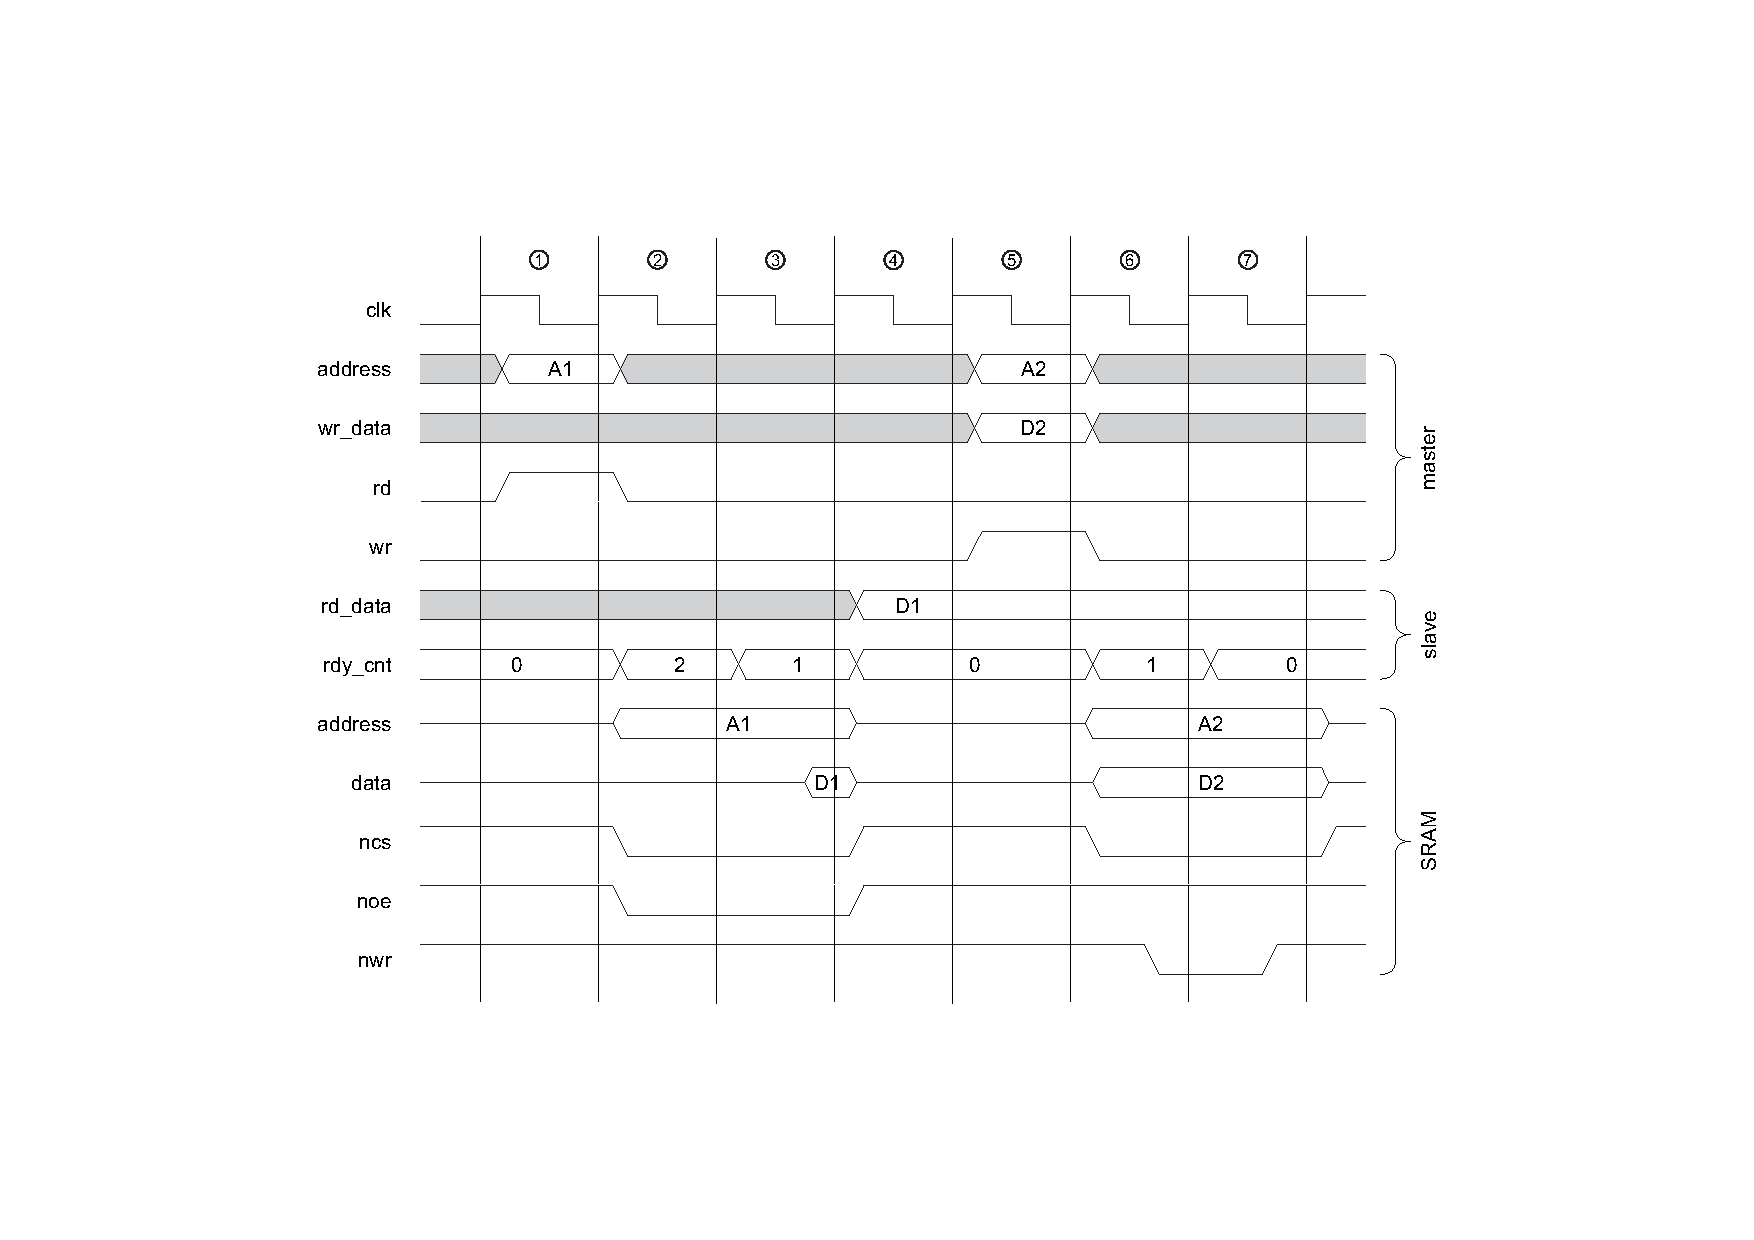
\includegraphics[scale=\scgrsc]{\scgrp/sc_sram}
    \caption{Static RAM interface without pipelining}
    \label{fig:sc:sram}
\end{figure}

In cycle~1 the read transaction is started by the master and the
slave registers the address. The slave also sets the registered
control signals \sign{ncs} and \sign{noe} during cycle~1. Due to the
placement of the registers in the IO cells, the address and control
signals are valid at the FPGA pins very early in cycle~2. At the end
of cycle~3 (15~ns after \sign{address}, \sign{ncs} and \sign{noe}
are stable) the data from the RAM is available and can be sampled
with the rising edge for cycle~4. The setup time for the read
register is short as the register can be placed in the IO cell. The
master reads the data in cycle~4 and starts a write transaction in
cycle~5. Address and data are again registered by the slave and are
available for the RAM at the beginning of cycle~6. To perform a
write in two cycles the \sign{nwr} signal is registered by a
negative triggered flip-flop.

In Figure~\ref{fig:sc:sram:prd} we see a pipelined read from the RAM
with pipeline level 2. With this pipeline level and the two cycles
read access time of the RAM we achieve the maximum possible
bandwidth.

\begin{figure}
    \centering
    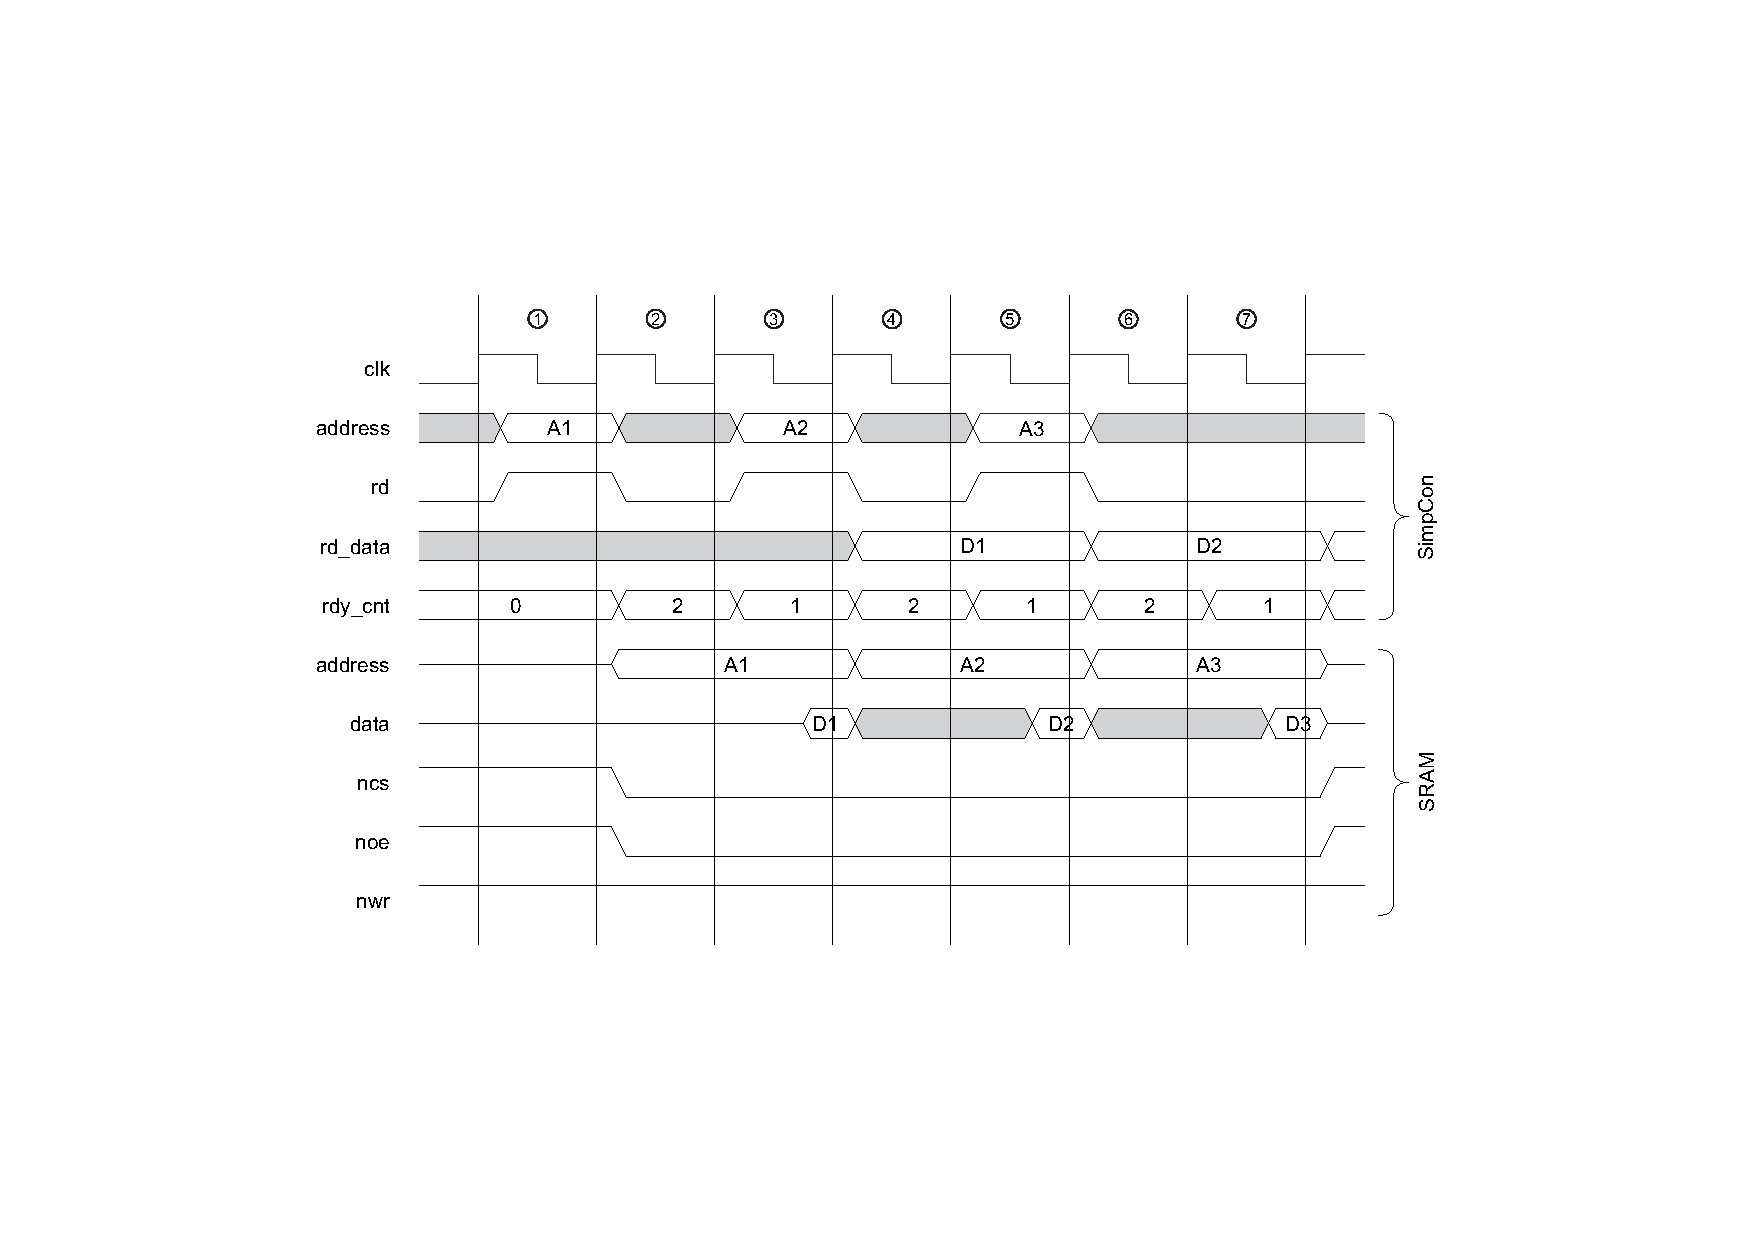
\includegraphics[scale=\scgrsc]{\scgrp/sc_sram_prd}
    \caption{Pipelined read from a static RAM}
    \label{fig:sc:sram:prd}
\end{figure}

We can see the start of the second read transaction in cycle 3
during the read of the first data from the RAM. The new address is
registered in the same cycle and available for the RAM in the
following cycle 4. Although we have a pipeline level of 2 we need no
additional address or data register. The read data is available for
two cycles (\sign{rdy\_cnt} 2 or 1 for the next read) and the master
is free to select one of the two cycles to read the data.

It has to be noted that pipelining with one read per cycle is
possible with SimpCon. We just showed a 2 cycle slave in this
example. For a SDRAM memory interface the ready counter will stay
either at 2 or 1 during the single cycle reads (depending on the
slave pipeline level). It will go down to 0 only for the last data
word to read.

\subsection{Master Multiplexing}

To add several slaves to a single master the \sign{rd\_data} and
\sign{bsy\_cnt} have to be multiplexed. Due to the fact that all
\sign{rd\_data} signals are registered by the slaves a single
pipeline stage will be enough for a large multiplexer. The selection
of the multiplexer is also known at the transaction start but needed
at most in the next cycle. Therefore it can be registered to further
speed up the multiplexer.
\ \\
\ \\
TODO: add a schematic for the master \sign{rd\_data} multiplexer.

\section{Available VHDL Files}

Besides the SimpCon documentation some example VHDL files for slave
devices and bridges are available from
\url{http://www.opencores.org/projects.cgi/web/simpcon/overview}.
All components are also part of the standard JOP distribution.


\subsection{Components}

\begin{itemize}
    \item \code{sc\_pack.vhd} defines VHDL records and some
    constants.
    \item \code{sc\_test\_slave} is a very simple SimpCon device. A
    counter to be read out and a register that can be written and
    read. There is no connection to the outer world. This example
    can be used as basis for a new SimpCon device.
    \item \code{sc\_sram16.vhd} is a memory controller for 16-bit
    SRAM.
    \item \code{sc\_sram32.vhd} is a memory controller for 32-bit
    SRAM.
    \item \code{sc\_sram32\_flash.vhd} is a memory controller for 32-bit
    SRAM, a NOR Flash, and a NAND Flash as used in the Cycore FPGA board for JOP.
    \item \code{sc\_uart.vhd} is a simple UART with configurable
    baud rate and FIFO width.
    \item \code{sc\_usb.vhd} is an interface to the parallel port of
    the FTDI 2232 USB chip. The register definition is identical to
    the UART and the USB connection can be used as a drop in
    replacement for a UART.
    \item \code{sc\_isa.vhd} interfaces the old ISA bus. It can be used
    for the popular CS8900 Ethernet chip.
    \item \code{sc\_sigdel.vhd} is a configurable sigma-delta converter
    for an FPGA that needs at minimum just two external components:
    a capacitor and a resistor.
    \item \code{sc\_fpu.vhd} provides an interface to the 32-bit FPU available
    at \url{www.opencores.org}.
    \item \code{sc\_arbiter.vhd} is a zero cycle latency, priority
    based SimpCon arbiter written by Christof Pitter \cite{jop:cmp}.
\end{itemize}

\subsection{Bridges}

\begin{itemize}
    \item \code{sc2wb.vhd} is a SimpCon/Wishbone \cite{soc:wishbone}
    bridge.
    \item \code{sc2avalon.vhd} is a SimpCon/Avalon \cite{soc:avalon}
    bridge to integrate a SimpCon based design with Altera's SOPC
    Builder \cite{quartus}.
    \item \code{sc2ahbsl.vhd} provides an interface to AHB slaves as
    defined in Gaisler's GRLIB \cite{grlib}. Many of the available
    GPL AHB modules from the GRLIB can be used in a SimpCon based
    design.
\end{itemize}


\section{Why a New Interconnection Standard?}

There are many interconnection standards available for SoC designs.
The natural question is: Why propose a new one? The answer is given
in the following section. For short: The available standards are
still in the tradition of backplane busses and do not fit very well
for pipelined on-chip interconnections.

\subsection{Common SoC Interconnections}


Several point-to-point and bus standards have been proposed over the
last years. The following section gives a brief overview of common
SoC interconnection standards.

The Advanced Microcontroller Bus Architecture (AMBA) \cite{soc:amba}
is the interconnection definition from ARM. The specification
defines three different busses: Advanced High-performance Bus (AHB),
Advanced System Bus (ASB), and Advanced Peripheral Bus (APB). The
AHB is used to connect on-chip memory, cache, and external memory to
the processor. Peripheral devices are connected to the APB. A bridge
connects the AHB to the lower bandwidth APB. An AHB bus transfer can
be one cycle with burst operation. With the APB a bus transfer
requires two cycles and no burst mode is available. Peripheral bus
cycles with wait states are added in the version 3 of the APB
specification. ASB is the predecessor of AHB and is not recommended
for new designs (ASB uses both clock phases for the bus signals --
very uncommon for today's synchronous designs). The AMBA 3 AXI
(Advanced eXtensible Interface) \cite{soc:amba3} is the latest
extension to AMBA. AXI introduces out-of-order transaction
completion with the help of a 4 bit transaction id tag. A ready
signal acknowledges the transaction start. The master has to hold
the transaction information (e.g.\ address) till the interconnect
signals ready. This enhancement ruins the elegant single cycle
address phase from the original AHB specification.

Wishbone \cite{soc:wishbone} is a public domain standard used by
several open-source IP cores. The Wishbone interface specification
is still in the tradition of microcomputer or backplane busses.
However, for a SoC interconnect, which is usually
point-to-point\footnote{Multiplexers are used instead of busses to
connect several slaves and masters.}, this is not the best approach.
The master is requested to hold the address and data valid through
the whole read or write cycle. This complicates the connection to a
master that has the data valid only for one cycle. In this case the
address and data have to be registered \emph{before} the Wishbone
connect or an expensive (time and resources) multiplexer has to be
used. A register results in one additional cycle latency. A better
approach would be to register the address and data in the slave. In
that case the address decoding in the slave can be performed in the
same cycle as the address is registered. A similar issue, with
respect to the master, exists for the output data from the slave: As
it is only valid for a single cycle the data has to be registered by
the master when the master is not reading it immediately. Therefore,
the slave should keep the last valid data at its output even when
the Wishbone strobe signal (\emph{wb.stb}) is not assigned anymore.
Holding the data in the slave is usually \emph{for free} from the
hardware complexity -- it is \emph{just} a specification issue. In
the Wishbone specification there is no way to perform pipelined read
or write. However, for blocked memory transfers (e.g. cache load)
this is the usual way to achieve good performance.


The Avalon \cite{soc:avalon} interface specification is provided by
Altera for a system-on-a-programmable-chip (SOPC) interconnection.
Avalon defines a great range of interconnection devices ranging from
a simple asynchronous interface intended for direct static RAM
connection up to sophisticated pipeline transfers with variable
latencies. This great flexibility provides an easy path to connect a
peripheral device to Avalon. How is this flexibility possible? The
\emph{Avalon Switch Fabric} translates between all those different
interconnection types. The switch fabric is generated by Altera's
SOPC Builder tool. However, it seems that this switch fabric is
Altera proprietary thus tying this specification to Altera FPGAs.

The On-Chip Peripheral Bus (OPB) \cite{soc:opb} is an open standard
provided by IBM and used by Xilinx. The OPB specifies a bus for
multiple masters and slaves. The implementation of the bus is not
directly defined in the specification. A distributed ring, a
centralized multiplexer, or a centralized AND/OR network are
suggested. Xilinx uses the AND/OR approach and all masters and
slaves must drive the data busses to zero when inactive.


Sonics Inc. defined the Open Core Protocol (OCP) \cite{soc:ocp} as
an open, freely available standard. The standard is now handled by
the OCP International Partnership (www.ocpip.org).




\subsection{What's Wrong with the Classic Standards?}

All SoC interconnection standards, that are widely in use, are still
in the tradition of a backplane bus. They force the master to hold
the address and control signals till the slave provides the data or
acknowledges the write request. However, this is not necessary in a
clocked, synchronous system. Why should we force the master to hold
the signals? Let the master move on after submitting the request in
a single cycle. Forcing the address and control valid for the
complete request disables any form of pipelined requests.


\begin{figure}
    \centering
    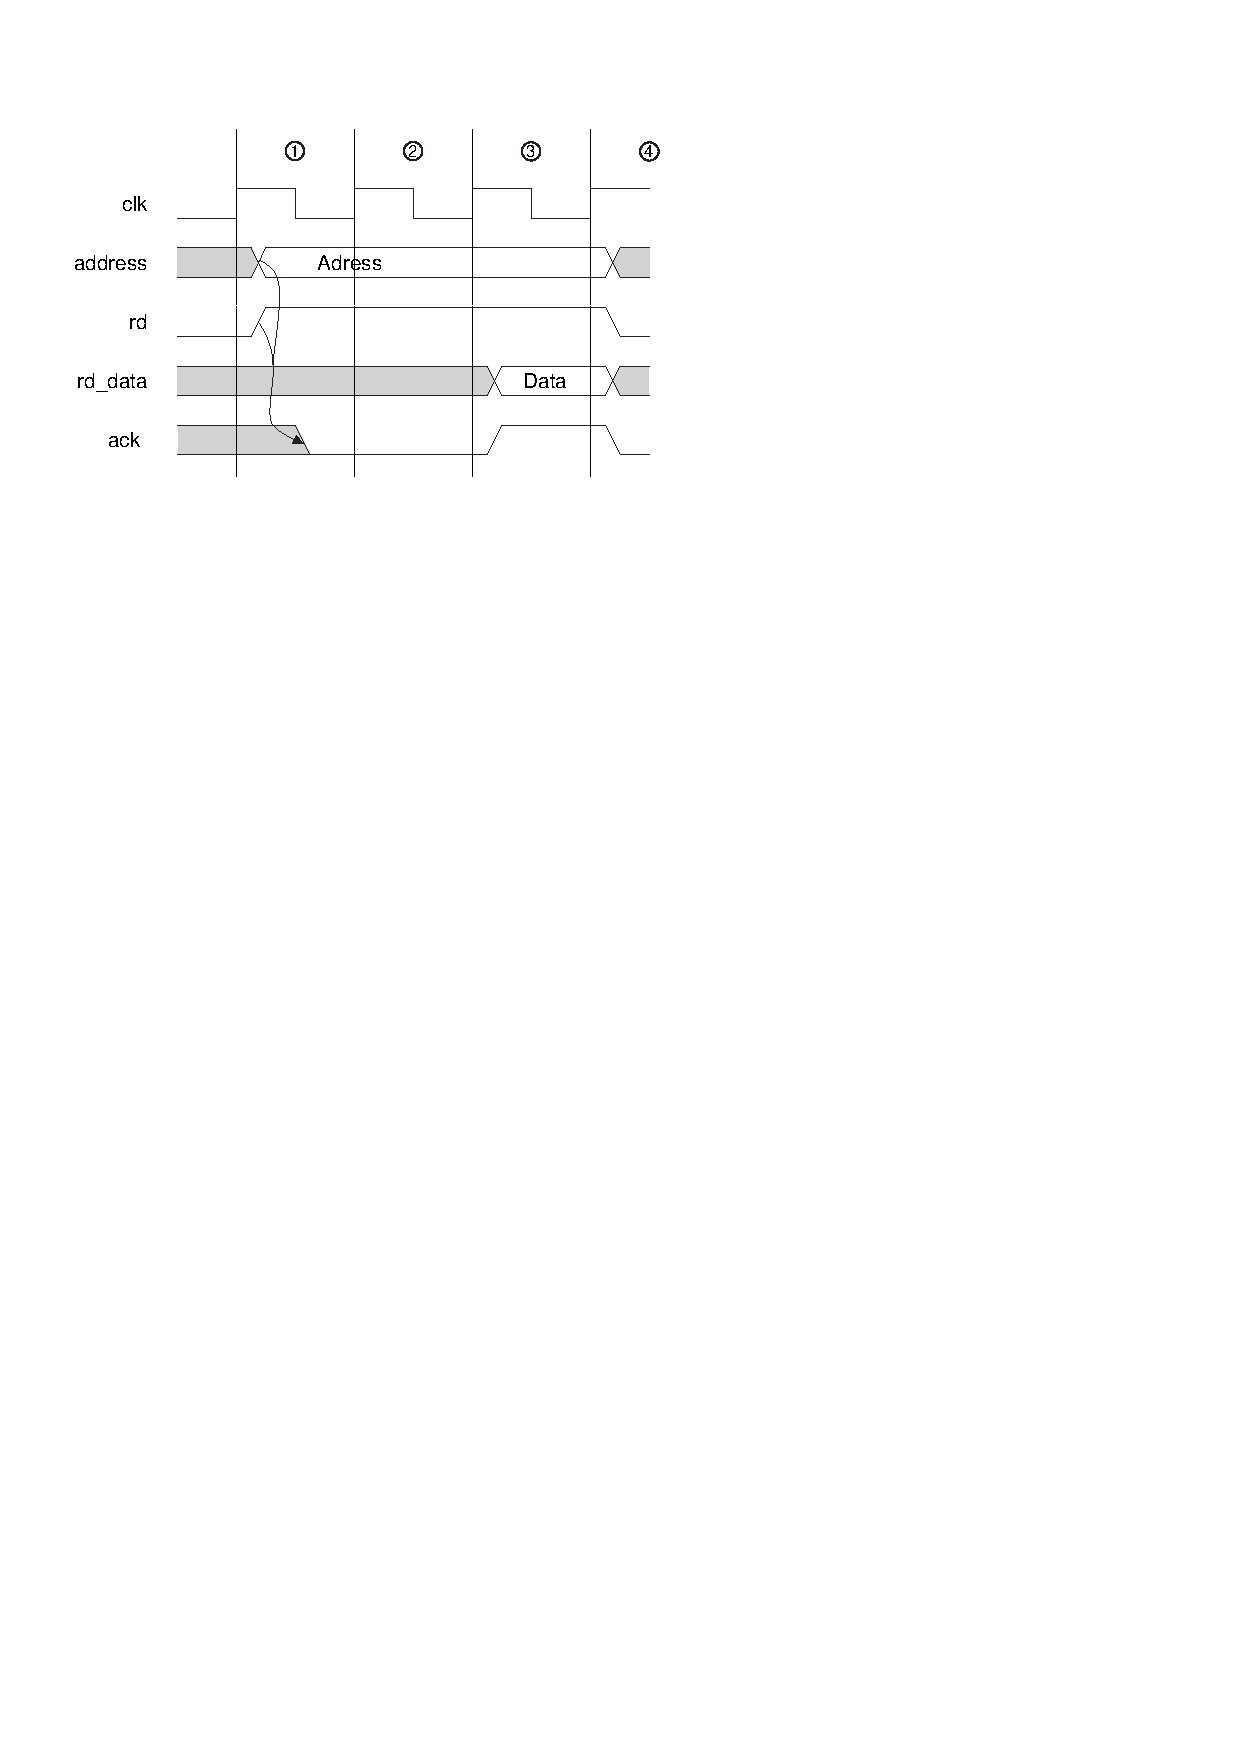
\includegraphics[scale=\scgrsc]{\scgrp/wb_basic_rd}
    \caption{Classic basic read transaction}
    \label{fig:wb:basic:rd}
\end{figure}

Figure~\ref{fig:wb:basic:rd} shows a read transaction with wait
states as defined in Wishbone \cite{soc:wishbone}, Avalon
\cite{soc:avalon}, OPB \cite{soc:opb}, and OCP
\cite{soc:ocp}\footnote{The signal names are different, but the
principle is the same for all mentioned busses.}. The master issues
the read request and the address in cycle 1. The slave has to reset
the \sign{ack} in the same cycle. When the slave data is available
the acknowledge signal is set (\sign{ack} in cycle 3). The master
has to read the data and register them within the same clock cycle.
The master has to hold the address, write data and control signal
active till the acknowledgement from the slave. For pipelined read
the \sign{ack} signal can be split into two signals (available in
Avalon and OCP): one to accept the request and a second one to
signal the available data.

The master is blind about the status of the outstanding transaction
until it is finished. It could be possible that the slave informs
the master in how many cycles the result will be available. This
information can help in building deeper pipelined masters.

Only the AMBA AHB \cite{soc:amba} defines a different protocol. A
single cycle address phase followed by a variable length data phase.
The slave acknowledgement (HREADY) is only necessary in the data
phase avoiding the combinatorial path from address/command to the
acknowledgement. Overlapping address and data phase is allowed and
recommended for high performance. Compared to SimpCon, AMBA AHB
allows for single stage pipelining, whereas SimpCon makes
multi-stage pipelining possible using the ready counter
(\sign{rdy\_cnt}). The \sign{rdy\_cnt} signal defines the delay
between the address and the data on a read, signalled by the slave.
Therefor, the pipeline depth of the bus and the slaves is only
limited by the bit width of \sign{rdy\_cnt}.


Another issue with all interconnection standards is the single cycle
availability of read data at the slaves. Why not keep the read data
valid as long as there is no new read data available? This feature
would allow the master to be more flexible when to read the data. It
would allow to issue a read command and then continue with other
instructions -- a feature known as data pre-fetching to hide long
latencies.

The last argument sounds contradictory to the first argument on
providing the transaction data at the master just for a single
cycle, but requesting the slave to hold the data for several cycles.
However, it is motivated to free up the master, keep it
\emph{moving}, and move the data hold (register) burden into the
slave. As data processing bottlenecks are usually found in the
master devices it sounds natural to move as much work as possible to
the slave devices to free up the master.

Avalon, Wishbone and OPB provide a single cycle latency access to
slaves due to the possibility to acknowledge a request in the same
cycle. However, this feature is a scaling issue for larger systems.
There is a combinatorial path from master address/command to address
decoding, slave decision on \sign{ack}, slave \sign{ack}
multiplexing back to the master and the master decision to hold
address/command or read the data and continue. Also the slave output
data multiplexer is on a combinatorial path from the master address.

AMBA AHB and SimpCon avoid this scaling issue by requesting the
acknowledge in the cycle following the command. In SimpCon and AMBA
the select for the read data multiplexer can be registered as the
read address is known at least one cycle before the data is
available. The later acknowledge results in a minor drawback on
SimpCon and AMBA (nothing is for free): It is not possible to
perform a single cycle read or write without pipelining. A single,
non pipelined transaction takes two cycles without a wait state.
However, a single cycle read transaction is only possible for very
simple slaves. Most non-trivial slaves (e.g.\ memory interfaces)
will not allow a single cycle access anyway.

\subsection{Evaluation}

We compare the SimpCon interface with the AMBA and the Avalon
interface as two examples of common interconnection standards. As
evaluation example we interface an external asynchronous SRAM with a
tight timing. The system is clocked with 100 MHz and the access time
for the SRAM is 15 ns. Therefore, there are 5 ns available for
on-chip register to SRAM input and SRAM output to on-chip register
delays. As SoC we use an actual low-cost FPGA (Cyclone EP1C6
\cite{AltCyc} and a Cyclone II).

The master is a Java processor (JOP \cite{jop:thesis,
jop:jnl:jsa2007}). The processor is configured with 4~KB instruction
cache and 512 Byte on-chip stack cache. We run a complete
application benchmark on the different systems. The embedded
benchmark (\emph{Kfl} as described in \cite{jop:austrochip05}) is an
industrial control application already in production.


%For a different benchmark (a UDP/IP application with IP processing -
%lot of buffer access) the difference is larger.

\begin{table}
    \centering

    \begin{tabular}{rll}
        \toprule
        Performance &      Memory     & Interconnect \\
        \midrule
        16,633 &  32 bit SRAM & SimpCon \\

        14,259 &  32 bit SRAM & AMBA \\

        14,015 &  32 bit SRAM & Avalon/PTF \\
        13,920 &  32 bit SRAM & Avalon/VHDL \\
        15,762 & 32 bit on-chip & Avalon\\

        14,760 &  16 bit SRAM & SimpCon \\

        11,322 &  16 bit SRAM & Avalon \\


         7,288  & 16 bit SDRAM & Avalon \\


%        Kfl & UDP/IP   &  Memory     & Interconnect \\
%        \midrule
%        16,633 & 6,537 & 32 bit SRAM & SimpCon \\
%
%        14,015 &       & 32 bit SRAM & Avalon/PTF \\
%        13,920 &       & 32 bit SRAM & Avalon/VHDL \\
%
%        14,760 & 5,716 & 16 bit SRAM & SimpCon \\
%
%        11,322 & 4,302 & 16 bit SRAM & Avalon \\
%        15,762 & --    & 32 bit on-chip & Avalon\\
%
%
%         7,288 & 2,677 & 16 bit SDRAM & Avalon \\


        \bottomrule

    \end{tabular}
    \caption{JOP performance with different interconnection types}
    \label{tab:perf:diff}

%         5,630 & 2,140 &  50 MHz & 16 bit SRAM (relaxed timing) & Avalon \\
%         6,243 & 2,389 &  50 MHz & 16 bit SRAM & Avalon \\

\end{table}

Table~\ref{tab:perf:diff} shows the performance numbers of this
JOP/SRAM interface on the embedded benchmark. It measures
iterations/s and therefore higher numbers are better. One iteration
is the execution of the main control loop of the \emph{Kfl}
application. For a 32 bit SRAM interface we compare SimpCon against
AMBA and Avalon. SimpCon outperforms AMBA by 17\% and Avalon by
19\%\footnote{The performance is the measurement of the execution
time of the whole application, not only the difference between the
bus transactions.} on a 32 bit SRAM.

The AMBA experiment uses the SRAM controller provided as part of
GRLIB \cite{grlib} by Gaisler Research. We avoided writing our own
AMBA slave to verify that the AMBA implementation on JOP is correct.
To provide a fair comparison between the single master solutions
with SimpCon and Avalon the AMBA bus was configured without an
arbiter. JOP is connected directly to the AMBA memory slave. The
difference between the SimpCon and the AMBA performance can be
explained by two facts: (1) as with the Avalon interconnect, the
master has the information when the slave request is ready at the
same cycle when the data is available (compared to the
\sign{rdy\_cnt} feature); (2) the SRAM controller is conservative as
it asserts \sign{HREADY} one cycle later than the data is available
in the read register (\sign{HRDATA}). The second issue can be
overcome by a better implementation of the SRAM AMBA slave.


The Avalon experiment considers two versions: an SOPC Builder
generated interface (PTF) to the memory and a memory interface
written in VHDL. The SOPC Builder interface performs slightly better
than the VHDL version that generates the Avalon \sign{waitrequest}
signal. It is assumed that the SOPC Builder version uses fixed wait
states within the switch fabric.

We also implemented an Avalon interface to the single-cycle on-chip
memory. SimpCon is even faster with the 32 bit off-chip SRAM than
with the on-chip memory connected via Avalon. Furthermore, we also
performed experiments with a 16 bit memory interface to the same
SRAM. With this smaller data width the pressure on the
interconnection and memory interface is higher. As a result the
difference between SimpCon and Avalon gets larger (30\%) on the 16
bit SRAM interface. To complete the picture we also measured the
performance with an SDRAM memory connected to the Avalon bus. We see
that the large latency of an SDRAM is a big performance issue for
the Java processor.

\section{Summary}

This document describes a simple (with respect to the definition and
implementation) and efficient SoC interconnect. The novel signal
\sign{rdy\_cnt} allows an early signalling to the master when read
data will be valid. This feature allows the master to restart a
stalled pipeline earlier to react for arriving data. Furthermore,
this feature also enables pipelined bus transactions with a minimal
effort on the master and the slave side.

We have compared SimpCon quantitative with AMBA and Avalon, two
common interconnection definitions. The application benchmark shows
a performance advantage of SimpCon by 17\% over AMBA and 19\% over
Avalon interfaces to an SRAM.

SimpCon is used as the main interconnect for the Java processor JOP
in a single master, multiple salves configuration. SimpCon is also
used to implement a shared memory chip-multiprocessor version of
JOP. Furthermore, in a research project on time-triggered
network-on-chip \cite{jop:ttnoc} SimpCon is used as the
\emph{socket} to this NoC.

The author thanks Kevin Jennings and Tommy Thorn for the interesting
discussions about SimpCon, Avalon and on-chip interconnection in
general at the usenet newsgroup \texttt{comp.arch.fpga}.
